\section{Dimensionierung PID Regler nach Ziegler-Nichols}

\subsection{Parameterbestimmung}

\begin{figure}[h!]
	\centering
	\begin{subfigure}{0.475\textwidth}
		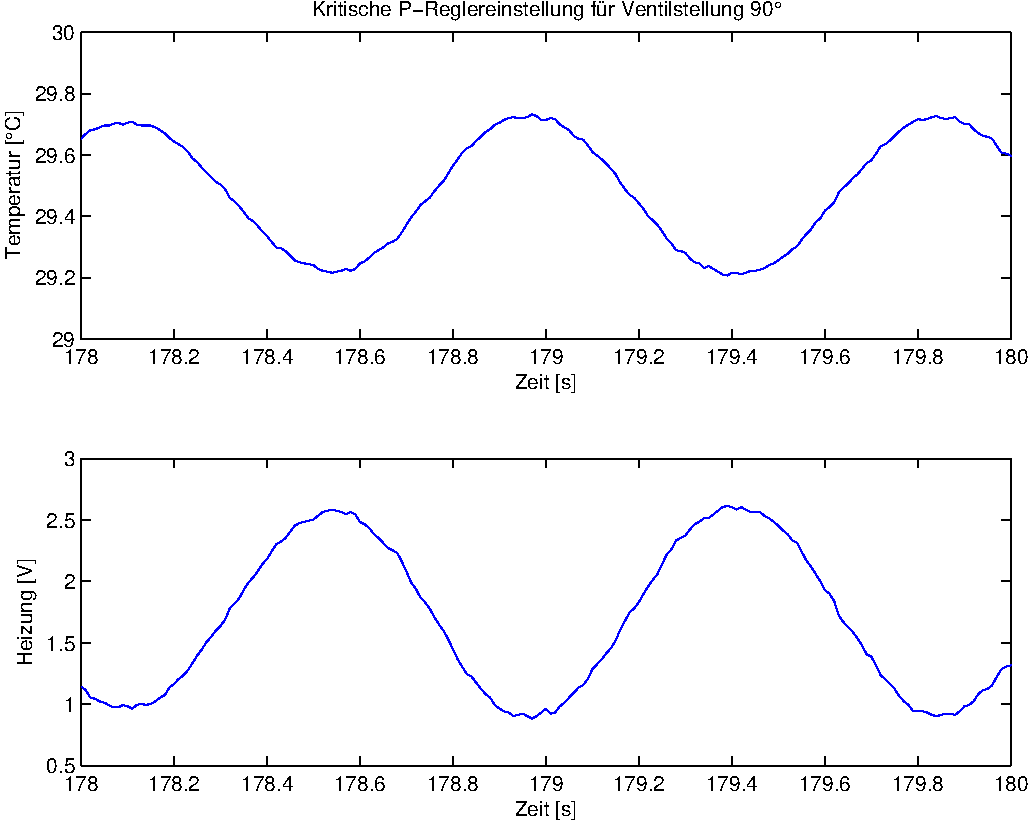
\includegraphics[width=1\textwidth]{06/p_krit_full_plot.pdf}
		\caption{Kritischer P-Regler für $\varphi = 90^\circ$}
	\end{subfigure}
	\hfill{}
	\begin{subfigure}{0.475\textwidth}
		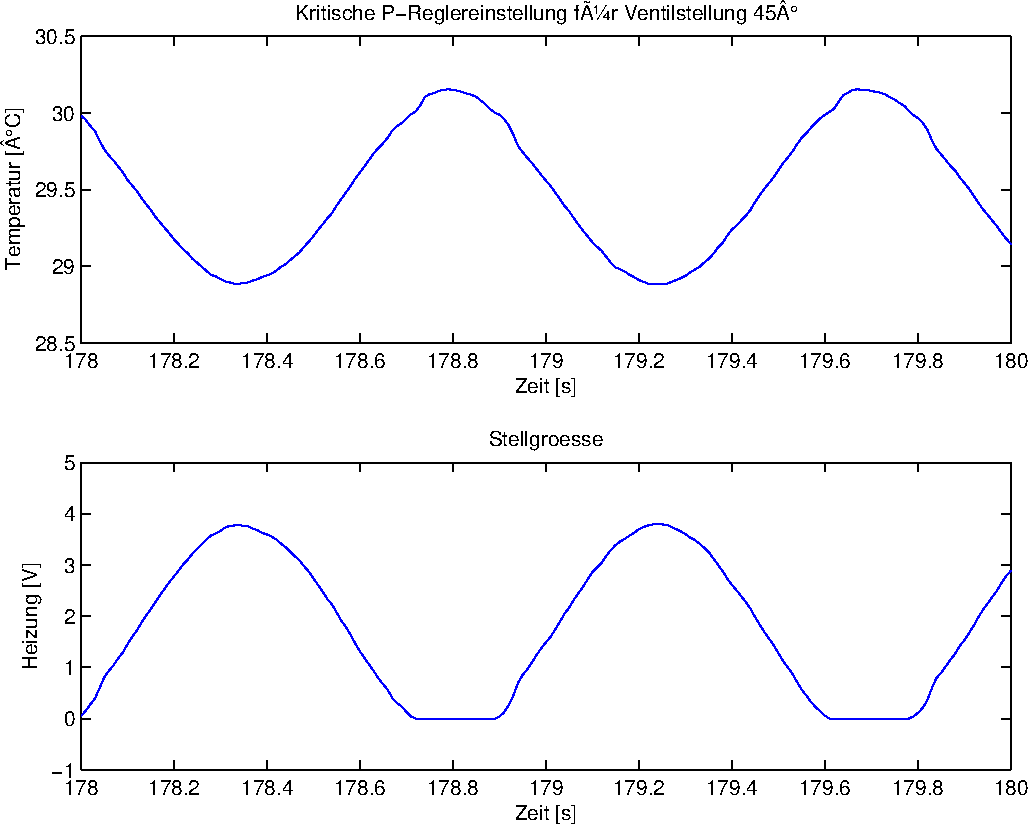
\includegraphics[width=1\textwidth]{06/p_krit_half_plot.pdf}
		\caption{Kritischer P-Regler für $\varphi = 45^\circ$}
	\end{subfigure}
	\caption{Messkurven für kritische P-Regler}
\end{figure}

Aus den Messdaten ergeben sich die folgenden Werte für den kritischen P-Regler
\begin{table}[h!]
	\centering
	\begin{tabular}{c c c c}
		Wert
			& $\varphi = 90^\circ$
			& $\varphi = 45^\circ$
			& Einheit \\
		\hline 
		$K_{p_{krit}}$
			& 3.3
			& 3.4
			& $\si[per-mode=fraction]{\volt\per\celsius}$ \\
		$T_{krit}$
			& 0.9
			& 0.8
			& $\si{\second}$
	\end{tabular}
\end{table}

Aus diesen Werten ergeben sich die folgenden PID-Regler 
\begin{table}[h!]
	\centering
	\begin{tabular}{c c c c c}
		Parameter
			& Berechnung
			& $\varphi = 90^\circ$
			& $\varphi = 45^\circ$
			& Einheit \\
		\hline
		$K_p$
			& $0.6 \cdot K_{p_{krit}}$
			& 1.98
			& 2.04
			& $\si[per-mode=fraction]{\volt\per\celsius}$ \\
		$T_n$
			& $0.5 \cdot T_{krit}$
			& 0.45
			& 0.4
			& $\si{\second}$ \\
		$T_v$
			& $0.125 \cdot T_{krit}$
			& 0.1125
			& 0.1
			& $\si{\second}$
	\end{tabular}
\end{table}

\subsection{Test des PID-Reglers}

\begin{figure}[h!]
	\centering
	\begin{subfigure}{0.475\textwidth}
		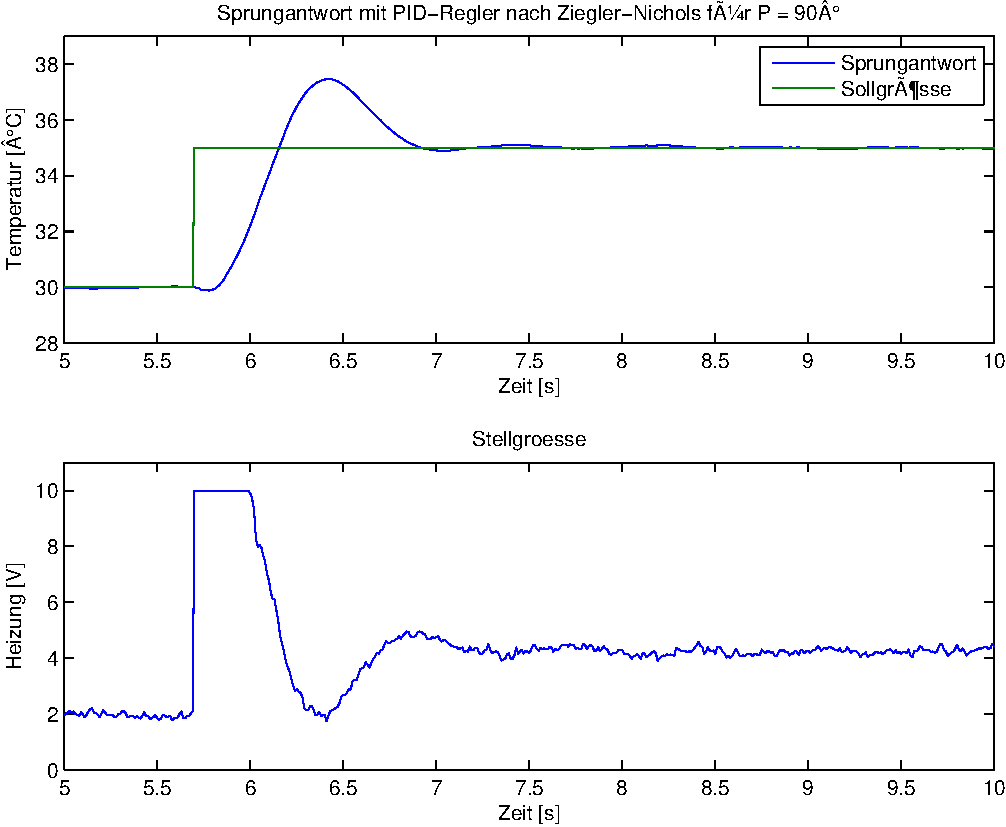
\includegraphics[width=1\textwidth]{06/pid_zn_full_plot.pdf}
		\caption{PID-Reglereinstellung für $\varphi = 90^\circ$}
	\end{subfigure}
	\begin{subfigure}{0.475\textwidth}
		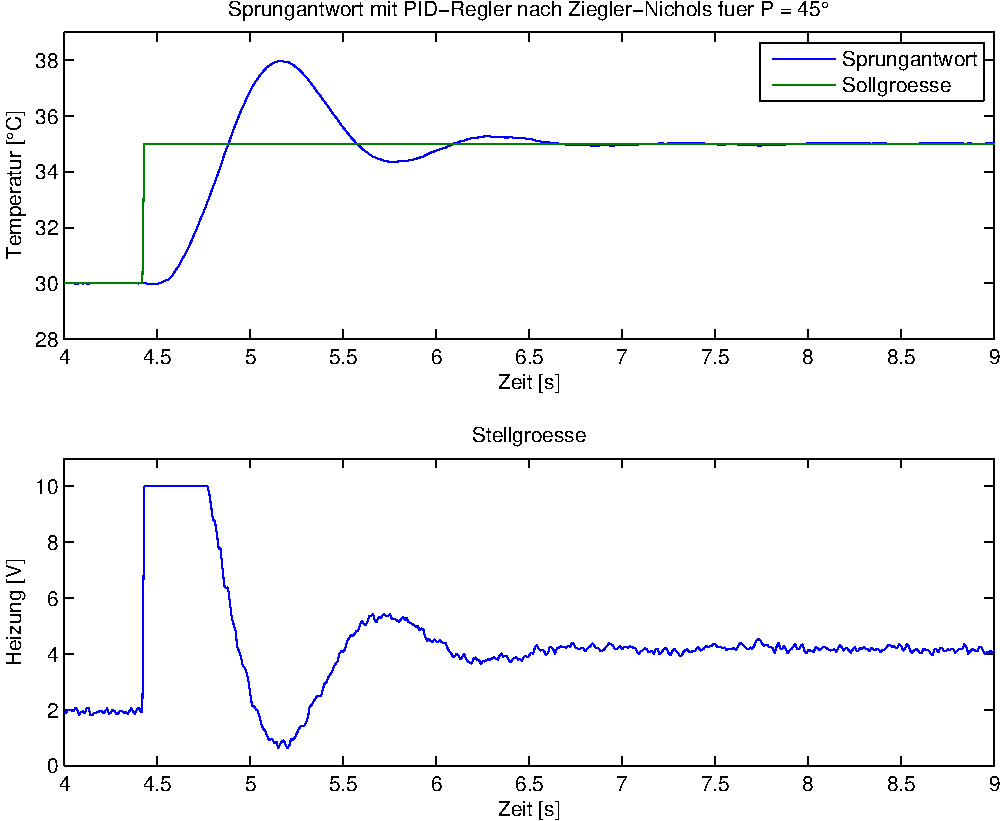
\includegraphics[width=1\textwidth]{06/pid_zn_half_plot.pdf}
		\caption{PID-Reglereinstellung für $\varphi = 45^\circ$}
	\end{subfigure}
	\caption{Sprungantworten der PID-Regler nach Ziegler-Nichols}
\end{figure}

\begin{table}[h!]
	\centering
	\begin{tabular}{l c c c}
		Eigenschaft
			& $\varphi = 90^\circ$
			& $\varphi = 45^\circ$ 
			& Einheit\\
		\hline
		Ausregelzeit ($e < 1\%$)
			& 2.7
			& 3.6
			& $\si{\second}$ \\
		Überschwingen
			& 49
			& 60
			& $\%$
	\end{tabular}
\end{table}
